\documentclass{eceasst}

\usepackage{minted}
\usepackage{subfig}

\usepackage{xcolor}
%\newcommand\todo[1]{\textcolor{red}{TODO #1}}

\input{frontmatter}

\usepackage{pdfcomment}
\newcommand{\todo}[1]{\pdfcomment[color={0.045 0.278 0.643},icon=Note]{#1}}

\title{Improving reproducibility of scientific software using Nix/NixOS: A case study on the preCICE ecosystem}
\short{preCICE on Nix: A case study}
\author{
Max Hausch\autref{1}\autref{*},
Simon Hauser\autref{1}\autref{*},
Benjamin Uekermann\autref{1}}

\institute{
\autlabel{1} Institute for Parallel and Distributed Systems\\ University of Stuttgart\\ \email{benjamin.uekermann@ipvs.uni-stuttgart.de}\\
%\autlabel{1} \email{st175425@stud.uni-stuttgart.de}\\
%\autlabel{2} \email{st148883@stud.uni-stuttgart.de}\\
\autlabel{*} These authors contributed equally to this work.}

\abstract{
Ensuring reproducibility of scientific software is crucial for the advancement of research and the validation of scientific findings.
However, achieving reproducibility in software-intensive scientific projects is often challenging due to dependencies, system configurations, and software environments.
In this paper, we present a possible solution for these challenges by utilizing Nix and NixOS.
Nix is a package manager and functional language, which guarantees that a package and all its dependencies can be built reproducibly.
NixOS is a purely functional Linux distribution, built on top of Nix, which enables the build of reproducible systems including configuration files, packages, and their dependencies.
We study the potential of Nix and NixOS by a case study on the reproducibility of the preCICE ecosystem.
preCICE is a coupling library for partitioned multiphysics simulations. The ecosystem includes diverse legacy solvers, adapters, and language bindings besides the coupling library itself making it a challenging and representative testcase.
We demonstrate how to create a reproducible and self-contained environment for this ecosystem and discuss the benefits and limitations of using Nix and NixOS.
%In addition, we compare the usability and reproducibility provided by Nix, in the context of preCICE, with two already established high-performance computing (HPC) solutions, Spack and EasyBuild.
%This evaluation enables us to assess the advantages and disadvantages of employing Nix to improve reproducibility in scientific software development within an HPC context.
}

\keywords{Reproducibility, Nix, NixOS, Spack, EasyBuild, preCICE, HPC}

\begin{document}
\maketitle

\section{Introduction}

In scientific research, it is crucial to be able to reproduce and verify results.
Reproducibility ensures that experiments can be repeated and findings can be validated, which is essential for reliable and credible research.
However, achieving reproducibility in scientific software has been a challenge due to complex dependencies, conflicting software environments, and changing software systems~\cite{Dalle_2012}.
Problems arise from dependencies, library versions, and system configurations, leading to inconsistencies across different computing environments.
Traditional approaches to reproducibility, such as manual setup instructions or virtualization techniques, are prone to errors and time-consuming at best.

Many scientists aim to solve this situation using Docker\footnote{\url{https://www.docker.com/}} (e.g.,\cite{koch2023sustainable}),
a software which describes software environments with the help of text files.
These text files are made up of imperative commands, which are run inside of containers, one layer at a time.
The result is several different layers combined into a single output image, which can be instantiated into a running container.
Docker images can be copied to different hosts and should then provide the same environment on different machines.
Those images are usually based on one of the official Docker images\footnote{\url{https://docs.docker.com/trusted-content/official-images/}}, however, which use traditional package managers, such as apt.
When a user then specifies to install the python3 package, for instance, a traditional package manager could yield version 3.8 today, but version 3.9 in a few months.
Full reproducibility can, thus, only be achieved by storing the complete image. Altering a single dependency (e.g., by a bugfix) causes a rebuild of the image and, thus, destroys reproducibility.

There are, moreover, commercial, domain specifig solutions to achieve reproducibility, e.g., CodeOcean\footnote{\url{https://codeocean.com/}} mainly for bioinformatics or Weights and Biases\footnote{\url{https://wandb.ai/site}} for machine learning.
With these archiving platforms, experiments can be rerun using technologies such as Docker.
The platforms are closed source, however, such that the source code cannot be reviewed nor adjusted~\cite{koch2023sustainable}.

In past years, the Nix package manager~\cite{Dolstra_2004} and NixOS~\cite{Dolstra_2010}, a Linux distribution built around it, have emerged as promising alternatives~\cite{Devresse_2015}.
Nix allows functional descriptions of dependencies up to fixed versions, thus avoiding the issue described above.
Similar ideas are followed by the popular high performance computing (HPC) package managers EasyBuild~\cite{easybuil6495863} and Spack~\cite{spack7832814}.
At FOSDEM 2018, Kenneth Hoste compares Spack, EasyBuild, and Nix with each other~\cite{Hoste}.
Minor deficits regarding reproducibility of Spack and EasyBuild are that they link against core system libraries, which can break independently. The Spack developers are aware of these shortcomings and are working on improvements\footnote{\url{https://github.com/spack/spack/issues/39560}}$^,$\footnote{\url{https://github.com/spack/spack/pull/42082}}.
EasyBuild, on the other hand, even has an option for linking against system libraries called \texttt{osdependencies}\footnote{\url{https://docs.easybuild.io/writing-easyconfig-files/\#dependency\_specs}}. Thus, packages need to be vetted and potentially updated prior to usage.
All three solutions have in common that they rely on scientific software following best practices concerning building and packaging.
Unfortunately, most legacy software projects do not do this.
This is why, for example, the xSDK community~\cite{xSDK2023} tries to set a standard for policies for math software.

In this paper, we analyze how well Nix and NixOS can improve reproducibility of scientific software.
To this end, we study the preCICE ecosystem~\cite{preCICEv2} as an example.
preCICE is a coupling library for partitioned multiphysics simulations.
The ecosystem includes diverse legacy solvers, adapters, language bindings, and tutorials besides the coupling library itself making it a challenging and representative testcase.
We try to build the complete ecosystem using Nix and run all tutorials.
This paper is the result of a student research project and a streamlined version of its report~\cite{studentreport}.

\section{Background}

This chapter gives a short introduction into Nix and preCICE.

\subsection{Nix}\label{sec:nix}

Nix is a purely functional package manager, which provides features to build software derivations reproducibly.
It does so, by recursively calculating a hash over all inputs of a derivation and its dependencies to ensure the completeness of the whole derivation.
If any of the inputs changes, all dependent derivations have to be rebuilt.
Fig.~\ref{fig:nix-graph} shows the dependency graph of the coreutils package as an example.

\begin{figure}
    \centering
    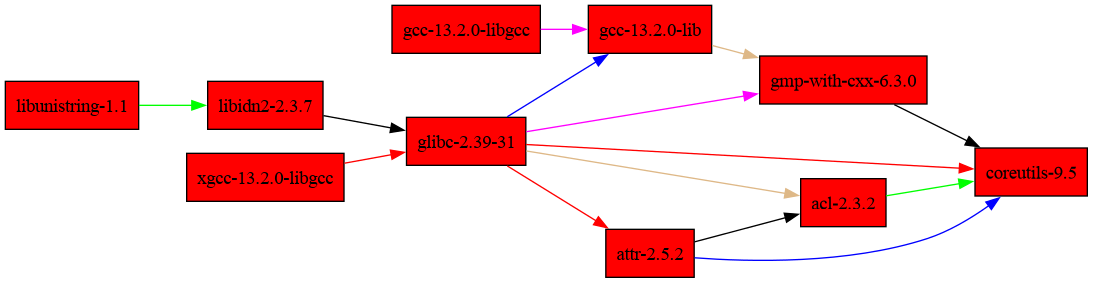
\includegraphics[width=1\textwidth]{figures/coreutils.png}
    \caption{The dependency graph of the coreutils package, generated by \texttt{nix-store --query --graph \$(nix build nixpkgs\#coreutils --print-out-paths) | dot -Tpng -Grankdir=LR -ocoreutils.png}}
    \label{fig:nix-graph}
\end{figure}

As Nix is purely functional, it relies on functions that, without side-effects, realize the package derivations.
Inputs of these functions are parameters such as the package version or the location of the source code.
Evaluating these functions with the same inputs yields the same outputs.
This is a critical factor for Nix's reproducibility.
Outputs, i.e. the build artifacts, never change after being built once.
Nix builds are, moreover, sandboxed, meaning that there is no internet access possible during a build.

All contents, including source files and resulting build artifacts, are stored inside the Nix store.
Per default, the Nix store resides in the path \texttt{/nix/store} on the file system.
The naming scheme for packages includes the above mentioned hash, for preCICE v2.5.0, for example,
\path{/nix/store/0a5gw3l...-precice-2.5.0}.
This eases checking the Nix store for integrity and ensures that builds using the same inputs are performed only once.
As all build outputs reference their complete dependency graphs inside the Nix store, they do not interfere with other build outputs, enabling installation of multiple versions of the same software without conflicts.

Software patches are easy to apply in Nix.
One can simply provide a list of \texttt{.patch} files as inputs, Nix then includes the patch files in the build and in the calculation of the hash.
Users can override all inputs, so that every package can be flexibly adjusted.


\subsection{preCICE}

preCICE (Precise Code Interaction Coupling Environment) is an open-source software library designed to facilitate coupling of different simulation software packages.
It provides an API, which allows different simulation tools to exchange data and work together in a collaborative manner, enabling multi-physics as well as multi-scale simulations.
In fact, many scientific simulations require complex combinations of multiple solvers, each specialized in a particular aspect of the problem.
For example, in fluid-structure interaction problems, where fluid flow interacts with deformable structures, separate solvers can be used to model the fluid dynamics and structural mechanics.

\begin{figure}
    \centering
    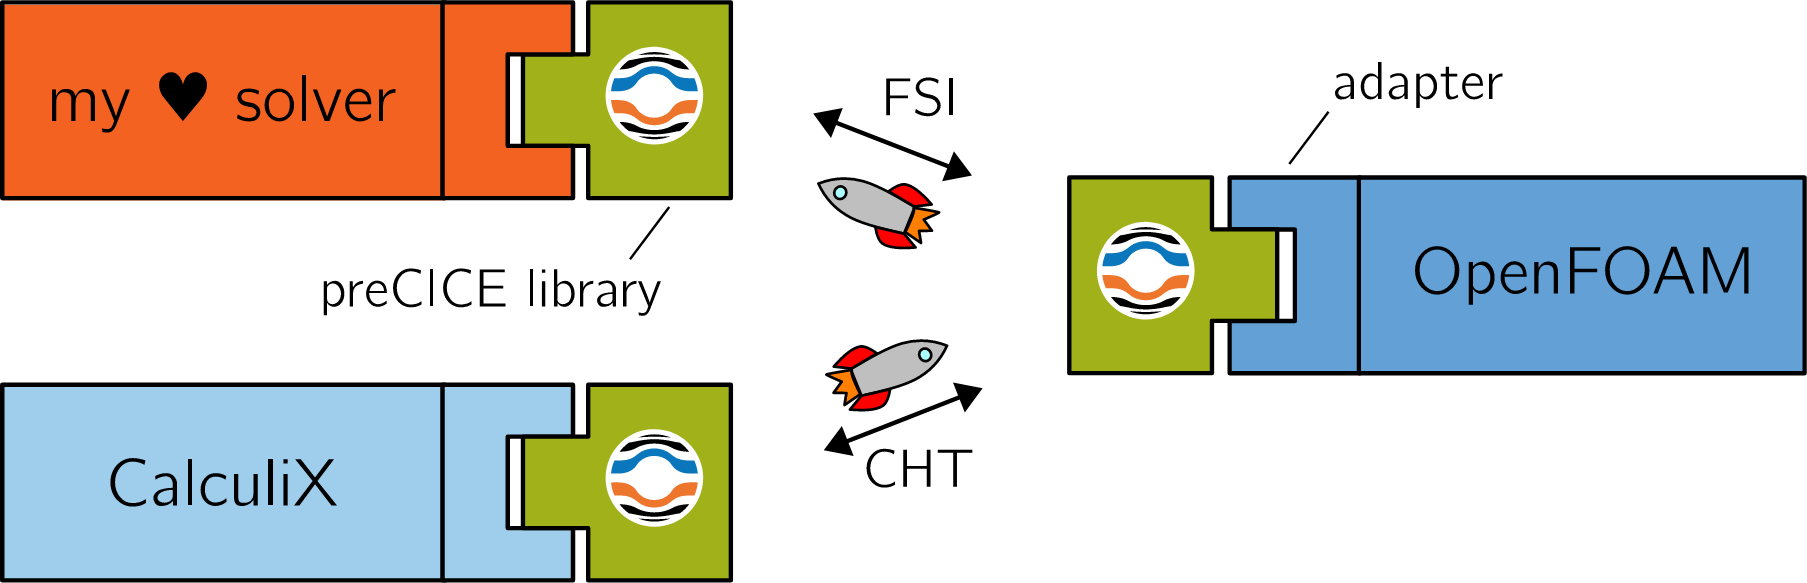
\includegraphics[width=0.5\textwidth]{figures/precice.png}
    \caption{Software setup of preCICE from the preCICE website \url{https://precice.org}}
    \label{fig:precice}
\end{figure}

preCICE supports a wide range of existing (Legacy) solvers. For each solver, there is typically a specific adapter: an either independent software package or simply a source code patch that integrates the preCICE API into the solver, see Fig.~\ref{fig:precice}.
The preCICE library itself is implemented in C++, bindings to other languages are either supported through native bindings (C, Fortran) or through independent software packages (Python, Julia, Matlab, Fortran).
Many official adapters, all bindings, the library itself, tutorials, additional tools, and the website including user documentation are collected and released in so-called preCICE distributions\footnote{\url{https://precice.org/installation-distribution.html}}.
In our case study, we target the distribution v2211.0~\cite{preciceDistribution}. To execute simulations, such as the included tutorials, requires the actual solvers next to the distribution. These are included, for example, in the preCICE VM\footnote{\url{https://precice.org/installation-vm.html}} and also part of our case study. Table \ref{table:label-distribution} lists all software packages of the case study. We try to reproducibly build all of these packages with Nix and try to run all tutorial cases.
The diverse languages and diverse solver packages using various build system makes the preCICE ecosystem a challenging testcase, which is, however, representative for current research software in our experience.


\begin{table}[!t]
  \normalsize
  \caption{Software packages of the case study}
  \label{table:label-distribution}
  \centering
  \begin{tabular}{|l|l|l|l|}
    \hline
    \bfseries Package & \bfseries Type & \bfseries Build system & \bfseries Version \\ \hline
    preCICE & library & cmake & 2.5.0 \\ \hline
    Fortran module & bindings & make & 9e3f405 \\ \hline
    Julia bindings & bindings & julia & 2.5.0 \\ \hline
    MATLAB bindings & bindings & matlab build script & 2.5.0.0 \\ \hline
    Python bindings & bindings & setup.py & 2.5.0.1 \\ \hline
    ASTE & tooling & cmake & 3.0.0 \\ \hline
    Config visualizer & tooling & setup.py & 60f2165 \\ \hline
    preCICE-CalculiX adapter & solver + adapter & makefile & 2.20 \\ \hline
    Code\_Aster & solver & custom system in python & 14.6.0 \\ \hline
    Code\_Aster-preCICE adapter & adapter & custom system in python & ce995e0 \\ \hline
    deal.II & solver & cmake & 9.4.1 \\ \hline
    preCICE-deal.II adapter & adapter & cmake & dbb25bea \\ \hline
    DUNE-FEM & solver library & setup.py & 2.8.0 \\ \hline
    preCICE-DUNE adapter& adapter & scripts + cmake & 5f2364d \\ \hline
    FEniCS & solver library& cmake + setup.py & 2019.1.0 \\ \hline
    preCICE-FEniCS adapter & adapter & setup.py & 1.4.0 \\ \hline
    Nutils & solver library & setup.py & 7.0.0 \\ \hline
    OpenFOAM & solver & wmake/Allwmake & 2206 \\ \hline
    preCICE-OpenFOAM adapter & adapter & wmake/Allwmake & 1.2.1 \\ \hline
    preCICE-SU2 adapter & solver + adapter & patch script + autoconf & 6.0.0 \\ \hline
  \end{tabular}
\end{table}


\section{Results}

We present challenges, solutions, and workarounds for packaging all components of the preCICE ecosystem.
The Nix code for all components is available online\footnote{\url{https://github.com/precice/nix-packages/}}.

\subsection{preCICE}

The preCICE library itself is already available in the nixpkgs repository\footnote{\url{https://github.com/NixOS/nixpkgs}}, so we do not have to package the software.
Looking at the package definition and the preCICE source code, the library is quite easy to build and package as it uses CMake as a build system.

\subsection{Tools}

The preCICE distribution includes several tools around preCICE.

\subsubsection{ASTE}

ASTE\footnote{\url{https://github.com/precice/aste}} stands for Artificial Solver Testing Environment. It is a thin wrapper around the preCICE API, which allows, for instance, testing of data mapping with real geometries.
ASTE requires VTK9\footnote{\url{https://vtk.org/}}, a visualization toolkit, which is built without python support in the nixpkgs repository to reduce compilation time.
This feature is needed for ASTE, however.
As already mentioned, Nix allows overriding of inputs, so in this case, we can look at the package definition of VTK.
The parameter \texttt{enablePython} can simply be set to \texttt{true}. We then also need to supply the version of python, which we set to python3.

\subsubsection{Config visualizer}

The preCICE config visualizer\footnote{\url{https://github.com/precice/config-visualizer}}, as the name suggests, visualizes preCICE configuration files. Similarly to preCICE itself, the tool is already packaged upstream.
As a python package, it is easy to handle with Nix.

\subsection{Bindings}

Bindings are used to offer interfaces to other programming languages.

\subsubsection{MATLAB bindings}

There were several attempts to package MATLAB\footnote{\url{https://de.mathworks.com/products/matlab.html}} for NixOS in the past\footnote{\url{https://github.com/NixOS/nixpkgs/issues/56887}}, yet there was no success so far.
This might be due to the fact, that MATLAB needs to be installed by running an installation wizard that downloads files during the installation process and verifies the licence.
Also, as MATLAB is not installed in the preCICE VM, we do not proceed in packaging the software.

\subsubsection{Fortran module}

We were able to package the Fortran module of preCICE by providing custom phases for the build phase and the install phase of Nix.
The resulting binary could run the example that comes with the module.

\subsubsection{Python bindings}

The \texttt{pyprecice} package is already available upstream, but did not compile as it is not able to find the python module \texttt{pkgconfig}.
After adding this single dependency as an input to the package definition, the python package builds and can be used as expected.
This solution was contributed to the upstream nixpkgs repository.

\subsubsection{Julia bindings}

Julia~\cite{bezanson2017julia} support in NixOS is currently still in its early stages and cannot be declaratively be defined by Nix\footnote{\url{https://github.com/NixOS/nixpkgs/issues/20649}}.

\subsection{Solvers and adapters}

\subsubsection{CalculiX}

The preCICE adapter for the structural mechanics code CalculiX~\cite{Uekermann2017_Adapters} requires the original CalculiX source code and provides a new makefile in the adapter repository.
By default, this makefile expects the source code to reside in \texttt{\$HOME}, but it is possible to override this location with a make variable.
It then builds the original code and the adapter code together, resulting in a combined binary.

The Makefile also has hard-coded locations of its dependencies: SPOOLES, ARPACK, and yaml-cpp. These need to be replaced with the equivalent pkg-config calls.
Additionally, there is no install target provided by the makefile, thus the resulting binary needs to be installed manually by copying it to \texttt{\$out}.

\subsubsection{Code\_Aster}

The Code\_Aster-preCICE adapter~\cite{Uekermann2017_Adapters} is a python file, which needs to be placed in the Code\_Aster lib directory.
For this, the Code\_Aster solver needs to be packaged at version 14.6.
It uses a custom build system based on a \texttt{setup.py} file, which invokes build and install phases for dependencies and in the end for the solver itself.

The Code\_Aster package distributes its dependencies as pinned tarballs.
On Nix, almost none of these dependencies complete the build stage. We, thus, need to pull them, package them separately as Nix packages, and configure the build system with a \texttt{setup.cfg}.
In this file, we are able to disable the installation of the pinned dependencies and provide paths to the dependencies instead.

More precisely, we disable HDF5, as it is already packaged in the upstream nixpkgs repository, even at the required version 5.1.10.
HDF5 is packaged with multiple outputs.
One package, \texttt{out}, contains the libraries and binaries and another, \texttt{dev} contains the header files, since most of the time, users installing HDF5 only need the libraries and binaries, and it helps to reduce installation size of this rather large package.
Additionally, Code\_Aster requires Medfile and Scotch, which are both available upstream and can be used as dependencies.
Another dependency is METIS, which partially builds. Thus, we decide to not replace it, but to fix the remainder of the build.
The issue is precisely that the \texttt{CMakeLists.txt} for the METIS programs hard-codes \texttt{link\_directories} to \path{/home/karypis/local/lib}. We unpack the METIS tarball, remove this line with sed, and repack the directory.

The remaining two dependencies, Mumps and Tfel are not available upstream and need to be packaged.
Mumps uses a Makefile and can be configured using Makefile.inc. By default, it provides a few configurations for systems such as Ubuntu. We use one of these provided configuration files to write our own custom config file.
It defines the locations for dependencies, such as Scotch, METIS, ParMETIS, or Blacs.
Almost all dependencies are available upstream, but we need to recompile Scotch with additional build flags.
Moreover, for packaging Blacs, which also uses a Makefile, we configure the build using a custom \texttt{Bmake.inc} file, which is used to set compiler flags, the path to MPI, and the bash installation.
Tfel, on the other hand, uses CMake as build system making it easy to package it with Nix.

After successfully packaging all dependencies, the build phase of Code\_Aster completes, but the installation part has another issue, which also affects new versions of Ubuntu and other distributions using a python version greater than 3.9.
There is a forum post\footnote{\url{https://forum.code-aster.org/public/d/26475-problem-installing-code-aster-version-14-6/11}} without resolution, so we need to manually patch the bug.
The issue is precisely, that the custom build system does not correctly calculate the python site-packages directory. It unconditionally slices the first 3 chars from \texttt{sys.version}, which works for version 3.9.x, but not for version 3.10.x.
After patching, Code\_Aster successfully installed into \texttt{\$out/14.6/}, so we move around some files until we have a valid directory structure with \texttt{\$out/bin}, \texttt{\$out/lib}, providing symlinks for \texttt{\$out/14.6/} and \texttt{\$out/stable/}.

\subsubsection{deal.II}


To package the deal.II-preCICE adapter, we first need to package deal.II~\cite{dealII95} itself, which uses CMake as build system and works without any adjustments.
The same then applies for the adapter, which also uses CMake.
As an example for the Nix language, we provide the Nix code for the deal.II-preCICE adapter in Fig.~\ref{lst:dealii-adapter-nix}.

\begin{figure*}
    \normalsize
    \begin{minted}{nix}
{ lib, stdenv, fetchFromGitHub, cmake, precice,
  dealii, enable3d ? false }:
stdenv.mkDerivation rec {
  pname = "precice-dealii-adapter";
  version = "unstable-2022-09-23";

  src = fetchFromGitHub {
    owner = "precice"; repo = "dealii-adapter";
    rev = "dbb25...8367c"; sha256 = "sha256-pPQ2...2jlflgUE=";
  };

  nativeBuildInputs = [ cmake ];
  buildInputs = [ precice dealii ];

  cmakeFlags = lib.optionals enable3d [ "-DDIM=3" ];

  installPhase = ''
    mkdir -p $out/bin && cp elasticity $out/bin/elasticity
  '';
}
    \end{minted}
    \caption{Nix code to package the deal.II-preCICE adapter}
    \label{lst:dealii-adapter-nix}
\end{figure*}

\subsubsection{DUNE}

DUNE~\cite{bastian2020dune} uses a combination of CMake files and custom build scripts making the build process in Nix tedious.
There is an ongoing migration from autotools to CMake for DUNE, which might improve the situation in the future.
Another minor issue is that the DUNE project is rather a collection of repositories than a monorepo. This means, users have to correctly clone all repositories such that the build system finds all relevant information.
We clone all of the required DUNE repositories into a directory and additionally clone the DUNE-preCICE adapter into the same directory.
For the build and install process, we need to manually set the \texttt{\$DUNE\_CONTROL\_PATH} and the \texttt{\$DUNE\_PY\_DIR} environment variables. Both variables also need to be set at runtime.
Additionally, we need to patch the python install process because the current CMake file tries to access the internet with \texttt{pip install}, which is not allowed in Nix's sandboxed builds.
The two environment variables must also be set at runtime.
This can be achieved by sourcing the \texttt{set-dune-vars} script, which we provide.

\subsubsection{FEniCS}

FEniCS~\cite{fenics} is already packaged upstream, however, not with all features the FEniCs-preCICE adapter~\cite{Rodenberg2021} relies on, in particular PETSc support and mshr, the FEniCS mesh generator.
This is why, we need to package PETSc4py, the python bindings package of PETSc, which is not available upstream.
The build process uses the internal \texttt{buildPythonApplication} build tool and runs successfully once we add the option \texttt{build\_src --force} to rebuild cython code and pin the cython version to \texttt{0.29.34}~\footnote{\url{https://gitlab.com/petsc/petsc/-/issues/1359}}.
We could not enable tests for PETSc4py, however, because they depend on OpenMPI and the network, which is not available within Nix's build sandbox.
Afterwards, we specify PETSc4py as dependency for FEniCS and enable the PETSc support.
Additionally, we need to recompile PETSc with additional features enabled that are not enabled by the upstream Nix package. These include ParMETIS, HYPRE and ScaLAPACK. We use \texttt{overrideAttrs}, a Nix feature that allows us to change an existing package.
Lastly, we also package mshr, so all required features for the adapter package are now are available.

Building the FEniCS-preCICE adapter is now directly possible with \texttt{buildPythonPackage}.
All but two of the adapter's tests run successfully, which means, however, that we need to disable the tests.

\subsubsection{OpenFOAM}

The preCICE-OpenFOAM adapter~\cite{OpenFOAMpreCICE} supports multiple flavors of OpenFOAM. We restrict our analysis to the OpenFOAM fork of OpenCFD Ltd\footnote{\url{https://www.openfoam.com/}}.

OpenFOAM uses its own custom build system called \texttt{wmake}, which is typically called with a \texttt{Allwmake} wrapper script.
The build system sets 36 environment variables, one step at a time by checking several parameters, e.g.~the CPU architecture or the location of the source code. Also during runtime, these variables need to be set, either by a wrapper script or by manually sourcing a file inside the installation directory of OpenFOAM.
For Nix, these properties are unfortunate. To compile OpenFOAM with Nix, we need to patch the shebangs\footnote{\url{https://foldoc.org/shebang}} of wmake to make it run during the build.
We also use a shell script, which exports the environment variables to the current shell session.
For simplicity, we hard-code all parameters, such as the processor architecture. These could be parametrized, however, based on the Nix inputs to allow for optimized builds. We use the script during the build phase to source all variables such that, for example, \texttt{OPENFOAM\_SRC\_PATH} points to the default location \texttt{/build/openfoam}.
Afterwards, \texttt{./Allwmake -j -q} is sufficient to start the build.
The install phase then copies the necessary files and directories to \texttt{\$out}, replaces the mock \texttt{OPENFOAM\_SRC\_PATH} by the value of \texttt{\$out}, and creates a wrapper for the \texttt{openfoam} shell script.

The preCICE-OpenFOAM adapter is an OpenFOAM function object, requiring OpenFOAM and wmake as build inputs.
The environment variables have to be set again through the shell script mentioned above.
Afterwards, we set the target directory for the adapter to \texttt{\$out/lib/} as the adapter is a shared library. Building then works successfully.

\subsubsection{SU2}

The SU2-preCICE adapter~\cite{Uekermann2017_Adapters} patches and extends the original CFD code SU2~\cite{su2}.
To this end, the adapter provides a script to run before the build phase.
We do this in Nix' patch phase. Afterwards, \texttt{stdenv} automatically recognizes that SU2 uses autotools for building and runs the configure phase.
Finally, to find the preCICE installation, we need to set the configuration flags \texttt{--with-include} and \texttt{--with-lib}.

\subsubsection{Nutils}

The Nutils~\cite{nutils} solver can be build using \texttt{buildPythonPackage}. One test needs to be disabled, but the rest of the testsuite passes without issues. There is no dedicated Nutils-preCICE adapter, but preCICE is typically directly called from Nutils application scripts. 

\subsection{preCICE VM}

The current preCICE VM\footnote{\url{https://precice.org/installation-vm.html}} is built on top of Vagrant\footnote{\url{https://www.vagrantup.com/}} using Ubuntu as a base image.
When run for the first time, it further installs software, compiles programs, and clones the preCICE tutorials\footnote{\url{https://github.com/precice/tutorials/}}.
This inherently breaks reproducibility as the VM fetches files from the internet that are at this very point in time the \textit{latest} version, e.g. the \texttt{main} branch of the preCICE repository.

Nix comes with the built-in functionality of producing qemu\footnote{\url{https://www.qemu.org/}} VM images.
We use Nix to define a VM image with NixOS as a base, which can be built reproducibly.
The image contains all components of the case study and some additional custom tools that can only be seen in the official VM, such as the \texttt{preciceToPNG} command.
Also, we generate an iso and a Vagrant VirtualBox file of the VM as additional outputs.

\subsection{preCICE tutorials}

The preCICE tutorials included in the distribution cannot only be used as reference examples on how to couple different solvers, but also to verify functionality of solver and adapter installations by executing them.
To this end, we execute all 23 tutorials of the distribution such that each participant option is at least run once. We do not compare results, but only test whether the cases complete.
We test inside the NixOS VM and also in an ad-hoc shell environment provided by the \texttt{nix develop} command. All tests pass except the \textit{Turek-Hron FSI3}, parts of the \textit{partitioned heat conduction}, parts of the \textit{perpendicular flap}, and the \textit{flow over heated plate steady state} cases.
We could not build swak4foam, an add-on to OpenFOAM, which is needed in the Turek-Hron FSI3 tutorial and the OpenFOAM participants of the partitioned heat conduction tutorial.
The official preCICE VM uses a prebuilt version of swak4foam, but also patching the prebuilt binary did not work.
The dependency is, however, no longer required in the v202404.0 release of the distribution.
We could, moreover, not package the third-party solids4foam solver, which is one of many options in the perpendicular flap tutorial. 
The flow over heated plate steady state tutorial requires Code\_Aster. Even though we manage to package the solver, we observe a segmentation fault at runtime when the python code tries to call a Fortran subroutine -- a problem we did not manage to debug.

% \begin{sloppypar}
% \end{sloppypar}

\section{Discussion}

After detailing the challenges of building and packaging all components of the preCICE ecosystem and running the tutorials as testcases, we want to discuss common points between these scientific software packages.
The required effort to package the individual components varies drastically. Major problems can be traced back to the build system.
Custom build systems require an disproportional amount of additional work to make them runnable on any system.
OpenFOAM and Allwmake are prime examples of this issue. Package managers have to understand a whole new build system for a single package -- a fact that is often ignored when considering the trade-off between maintaining a custom build system versus pivoting to an industry standard, such as CMake or autotools.
Such standard build tools generally provide interfaces for dependency management and optional features. This is often better than only documenting these, since documentation needs to be kept in sync with the underlying code.

The authors of xSDK\footnote{\url{https://xsdk.info/}} come to a similar conclusion.
They provide a list of package policies~\cite{xSDK2023}, which, for example, specify that packages must have an appropriate build system, which includes CMake and autoconf as examples.
If a package supports all policies, they can be added to the growing list of packages in xSDK.
It is no surprise that xSDK packages (e.g., PETSc, deal.II, or preCICE) are also easy to package with Nix.

The xSDK policies also requires portable installations. Several components in the preCICE ecosystem require installation into \texttt{\$HOME} or any required files to be located at specific locations. Both, the CalculiX-preCICE adapter and the SU2-preCICE adapter require the original source code to be present as they add new features on top or patch the source code.
The current solution of cloning the code at the specific location works, but it might be better to look into Git submodules. This would moreover allow pinning the version of the original code compared to only documenting it.

Finally, hard-coding libraries to \texttt{/usr/lib} and \texttt{/usr/include} might work on one system, but might make it hard or even impossible to install a package on a different system.
Configurable solutions, such as \texttt{pkg-config}, should always be preferred and work out of the box with common paths such as \texttt{/usr/lib}.

\section{Conclusion}

We investigated on whether Nix und NixOS are a potential solution to enable full reproducibility of research software environments. As a case study, we tried to package and test all components of the preCICE ecosystem -- a very heterogeneous set of legacy software packages, which is, however, representative for the state of research software today in our experience.

We were able to package nearly all components and run nearly all test cases showing the potential of Nix in the domain of scientific software. Many packages required workarounds, however, which might be difficult to achieve for none-experienced Nix users.
Nix also comes with a few peculiarities, which complicate workarounds.
In fact, every piece of software has to lie within \texttt{/nix/store} and each path therein is its own-isolated tree inspired by the Filesystem Hierarchy Standard (FHS).

Most problems, however, can be traced back to a lack of standardization in research software, especially regarding build systems.
Software packages that follow best practices for their programming language are also straightforward to package.
The xSDK initiative defined such standardization policies for math software. Components of the preCICE ecosystem that already adhere to this standard, were among the easiest ones to package -- even though xSDK  ultimately targets Spack and not Nix.

This paper is the result of a student research project and a streamlined version of its report~\cite{studentreport}. Beyond the content of this paper, the report also includes a detailed comparison of Nix to Spack and EasyBuild, and a discussion on how to use Nix on HPC systems.

\acknowledge{
We thankfully acknowledge the funding by the Deutsche Forschungsgemeinschaft (DFG, German Research Foundation) under Germany's Excellence Strategy EXC 2075 -- 390740016 and the support by the Stuttgart Center for Simulation Science (SimTech).
}


\bibliographystyle{eceasst}
\bibliography{paper}

\end{document}
